\section{Pendahuluan}
\subsection{Latar Belakang}
Digital to Analog Converter (DAC) adalah perangkat yang berfungsi untuk mengubah sinyal digital menjadi sinyal analog. 
Sinyal digital yang dihasilkan oleh komputer atau mikrokontroler Arduino harus dapat diubah menjadi sinyal analog untuk dapat digunakan dalam berbagai aplikasi, seperti penggunaan dalam sistem audio, pengukuran, dan lain-lain.
\\\\
Prinsip kerja DAC melibatkan proses penggunaan resistor yang berat sebelah (binary weighted resistors) atau jaringan resistor R-2R ladder untuk menghasilkan output analog yang sesuai dengan input digital. 
Metode ini memungkinkan DAC untuk menghasilkan sinyal analog yang akurat dengan menggunakan kombinasi bit-bit digital.
\\\\
Dalam sistem monitoring, DAC digunakan untuk mengubah sinyal digital dari sensor menjadi sinyal analog yang dapat diproses oleh sistem. 
Misalnya, dalam pengukuran suhu, sensor suhu menghasilkan sinyal digital yang kemudian dikonversi menjadi sinyal analog oleh DAC sebelum diproses oleh sistem. 
Hal ini menunjukkan bahwa DAC sangat penting dalam sistem monitoring untuk mengubah sinyal digital menjadi sinyal analog yang dapat diproses oleh komputer.
\\\\

\subsection{Maksud dan Tujuan}
Mengetahui dan membandingkan hasil dari digital to analog converter pada Arduino dan Osiloskop.

\subsection{Hasil yang diharapkan}
Mendapatkan kesimpulan perbandingan hasil digital to analog converter pada Arduino dan Osiloskop.
%===========================================================%
\section{Tugas Pendahuluan}
\begin{center}
	\colorbox{cyan!30}{\parbox{0.8\linewidth}{
    \begin{enumerate}
        \item Apa yang dimaksud dengan Simple Queue?
        \item Keuntungan apa yang bisa didapat jika diterapkan ke suatu network?
    \end{enumerate}}}
\end{center}

%===========================================================%
\section{Alat dan Bahan}
\begin{itemize}[label=$\bullet$, itemsep=-1pt, leftmargin=*]
	\item 1 Perangkat Osiloskop
	\item 1 Laptop
	\item 1 Arduino
	\item Software Arduino IDE
\end{itemize}

%===========================================================%
\section{Jangka Waktu Pelaksanaan}
Pemahaman dan konfigurasi 1 jam.

%===========================================================%
\section{Penjelasan dan Tahapan Konfigurasi}

%======================PERCOBAAN 1==========================%
\subsection{Percobaan 1}
\begin{center}
	\textbf{Memulai Arduino IDE}
    \begin{enumerate}
        \item Buka aplikasi Arduino IDE.
        \item Masukkan kode program untuk menjalankan DAC (Digital to Analog Converter) pada Arduino IDE.
        \begin{figure}[H]
			\centering
			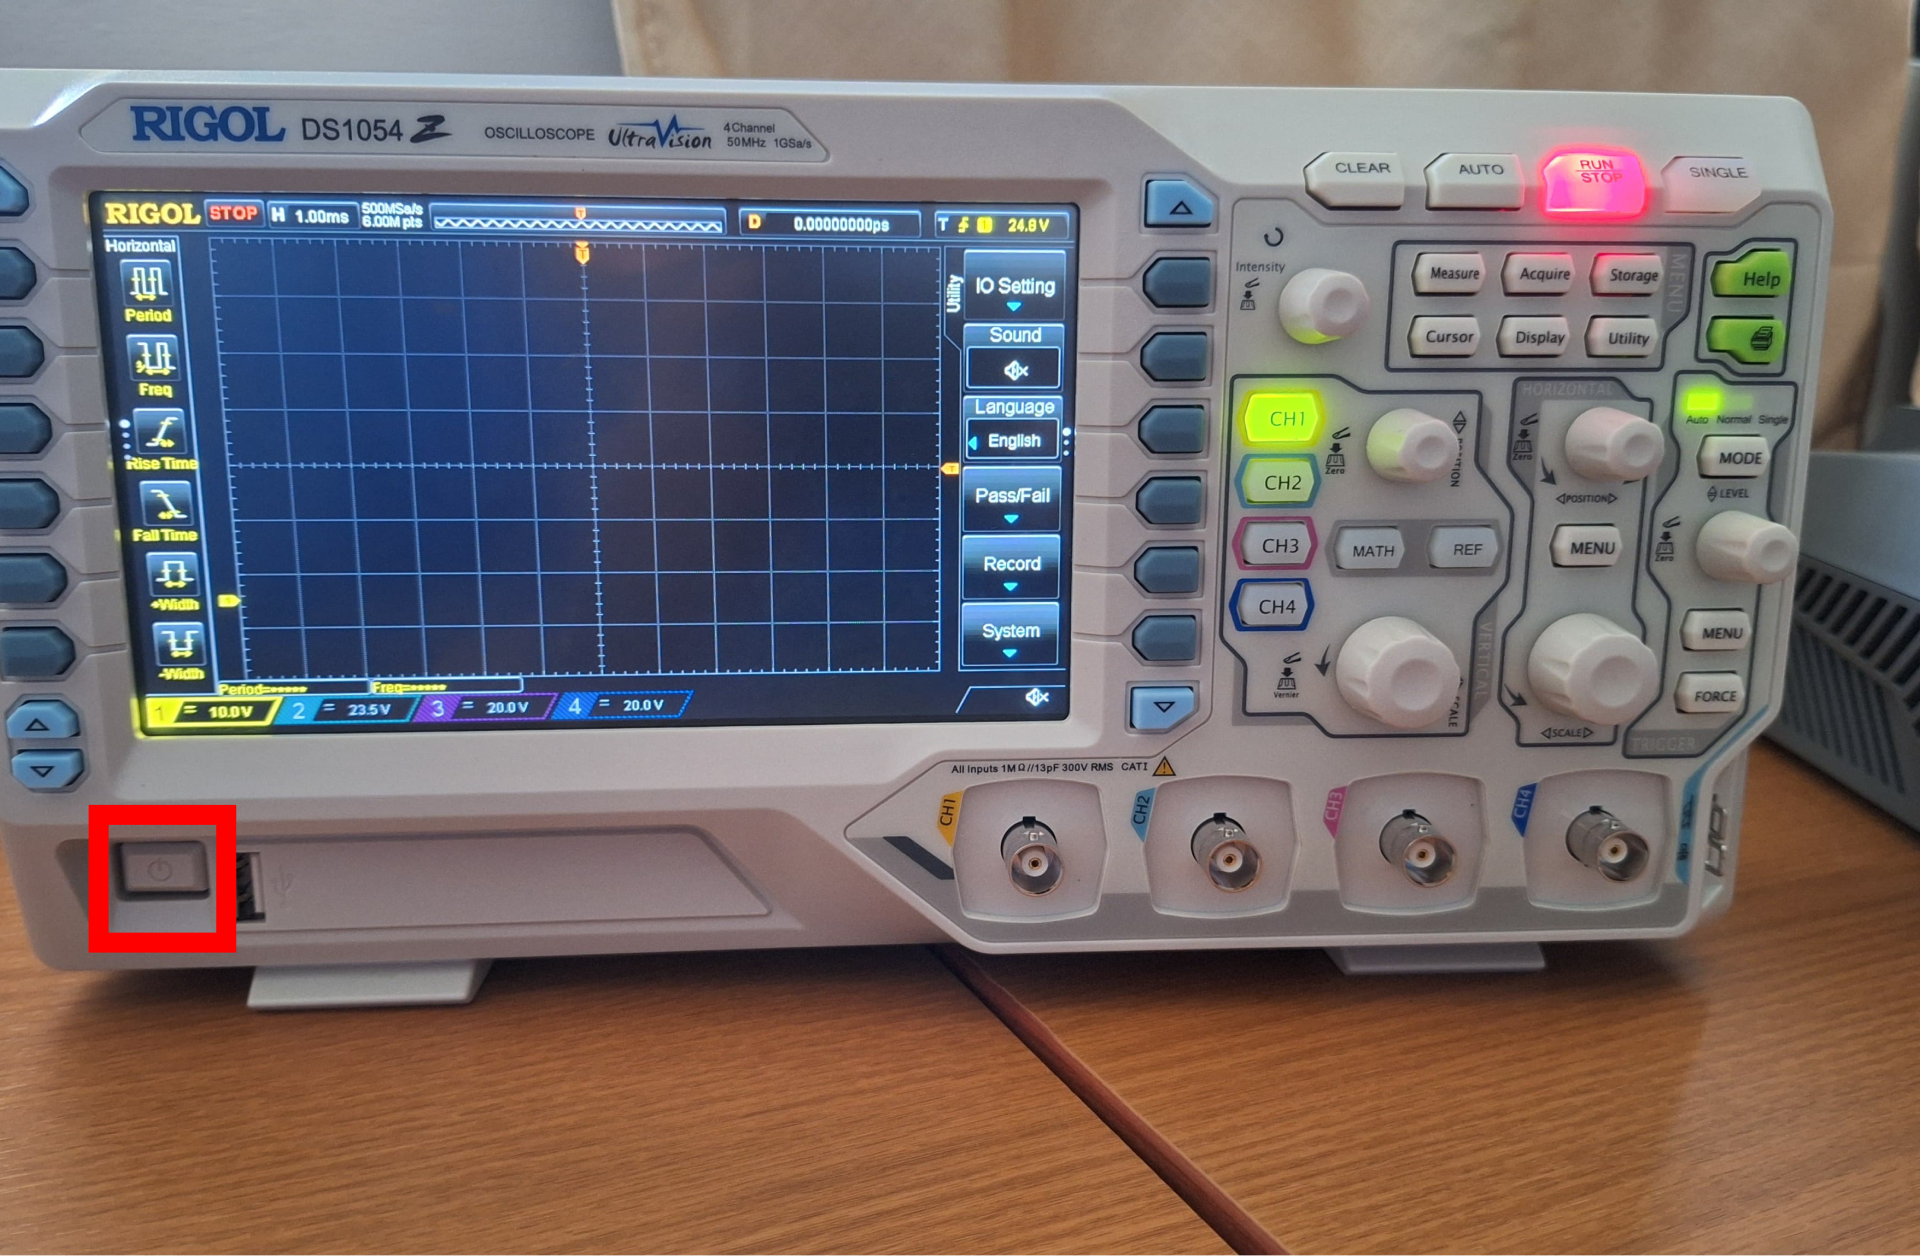
\includegraphics[width=0.8\linewidth]{P3/img/step 1.png}
			\caption{Step 1}
			\label{fig:Step 1}
		\end{figure}
		\item Hubungkan Arduino Uno dengan Arduino IDE.
        \begin{figure}[H]
			\centering
			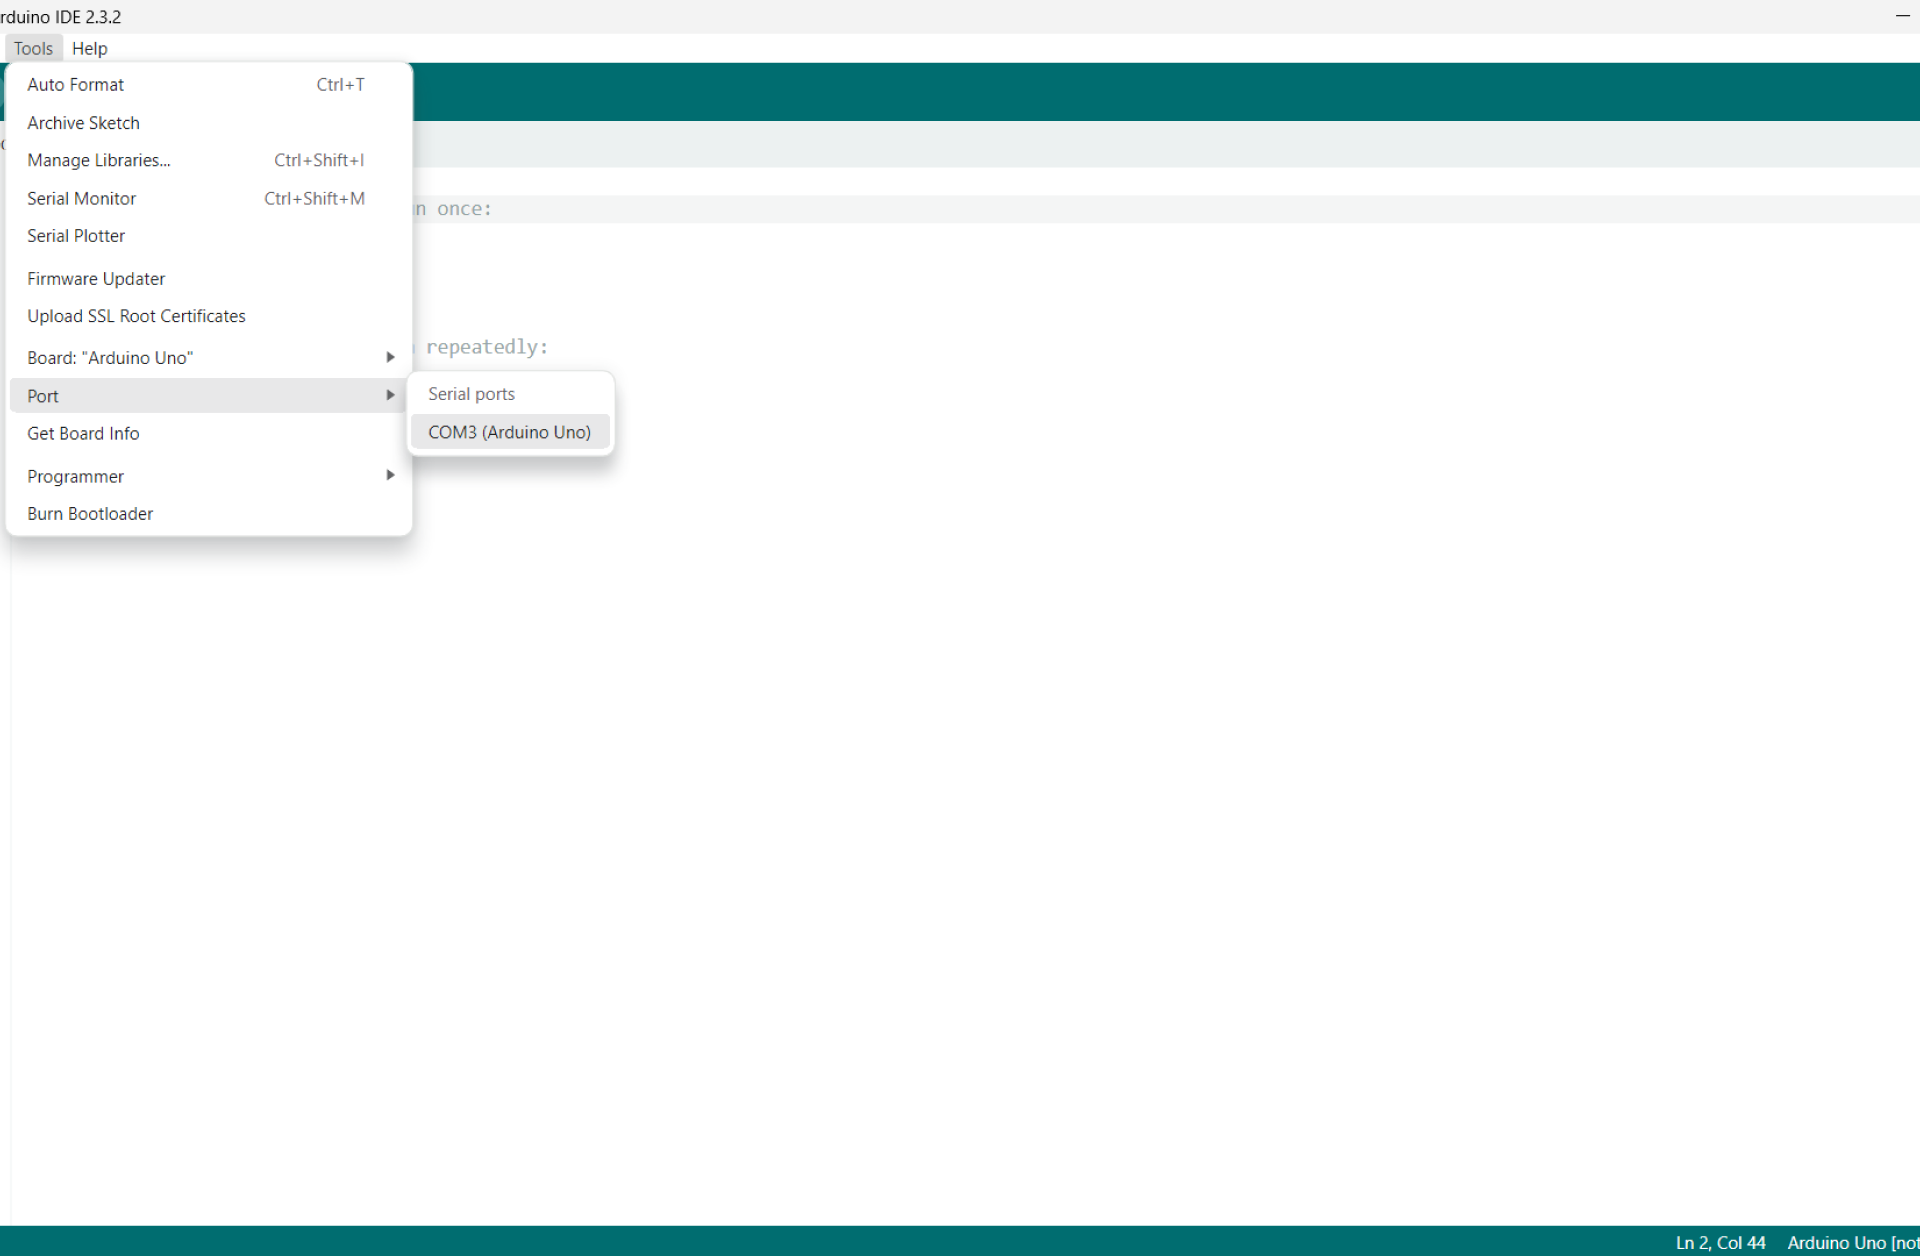
\includegraphics[width=0.8\linewidth]{P3/img/step 2.png}
			\caption{Step 2}
			\label{fig:Step 2}
		\end{figure}
        \item Buat rangkaian Arduino Uno dengan R2R Ladder seperti gambar dibawah ini.
        \begin{figure}[H]
			\centering
			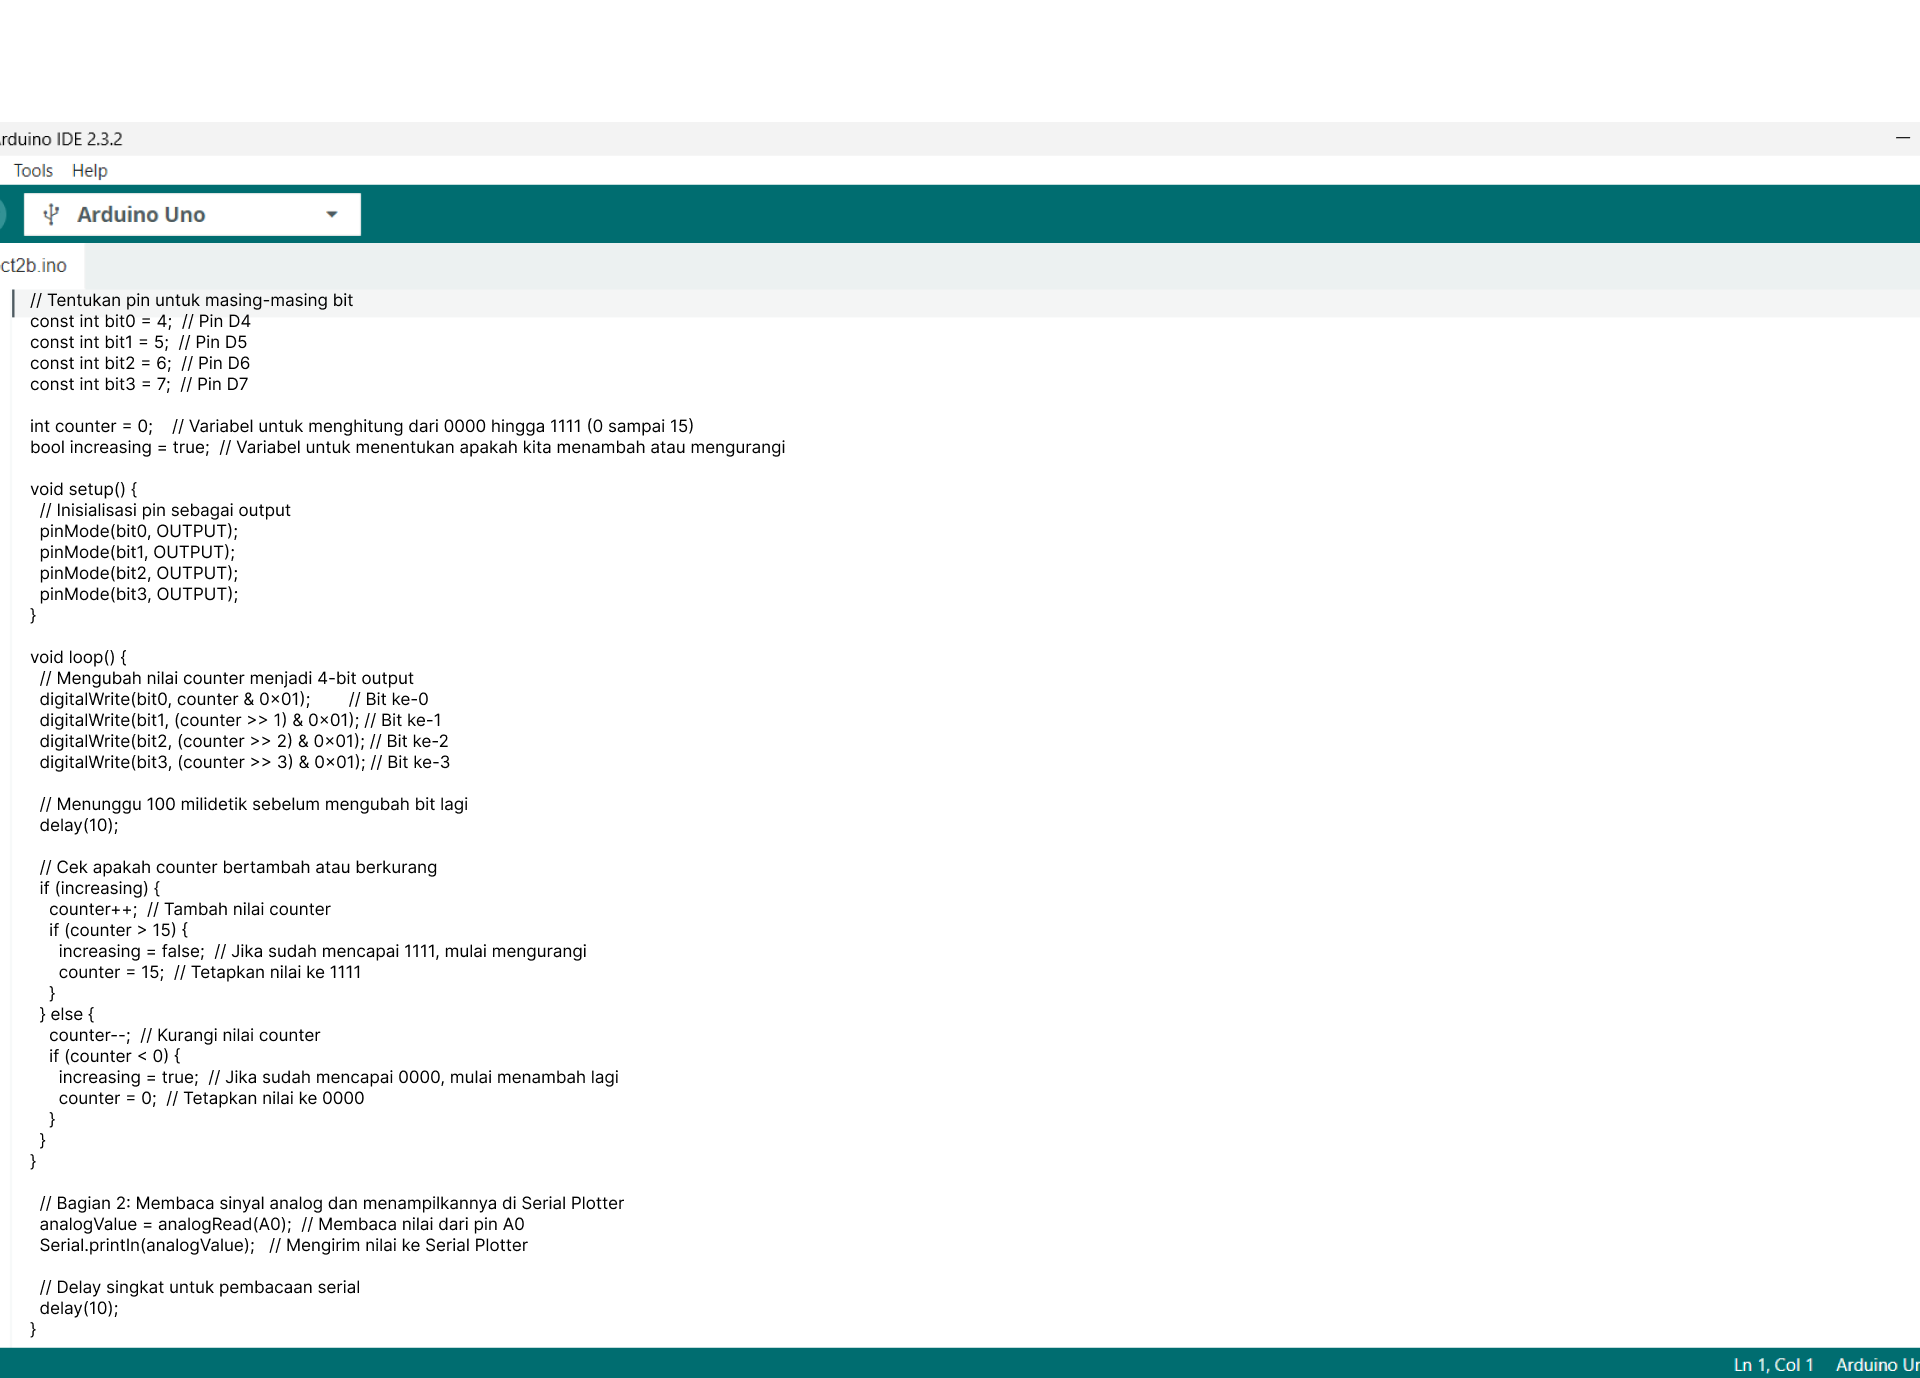
\includegraphics[width=0.8\linewidth]{P3/img/Step 3.png}
			\caption{Step 3}
			\label{fig:Step 3}
		\end{figure}
        \item Klik Verify, apabila berhasil maka klik upload.
        \begin{figure}[H]
			\centering
			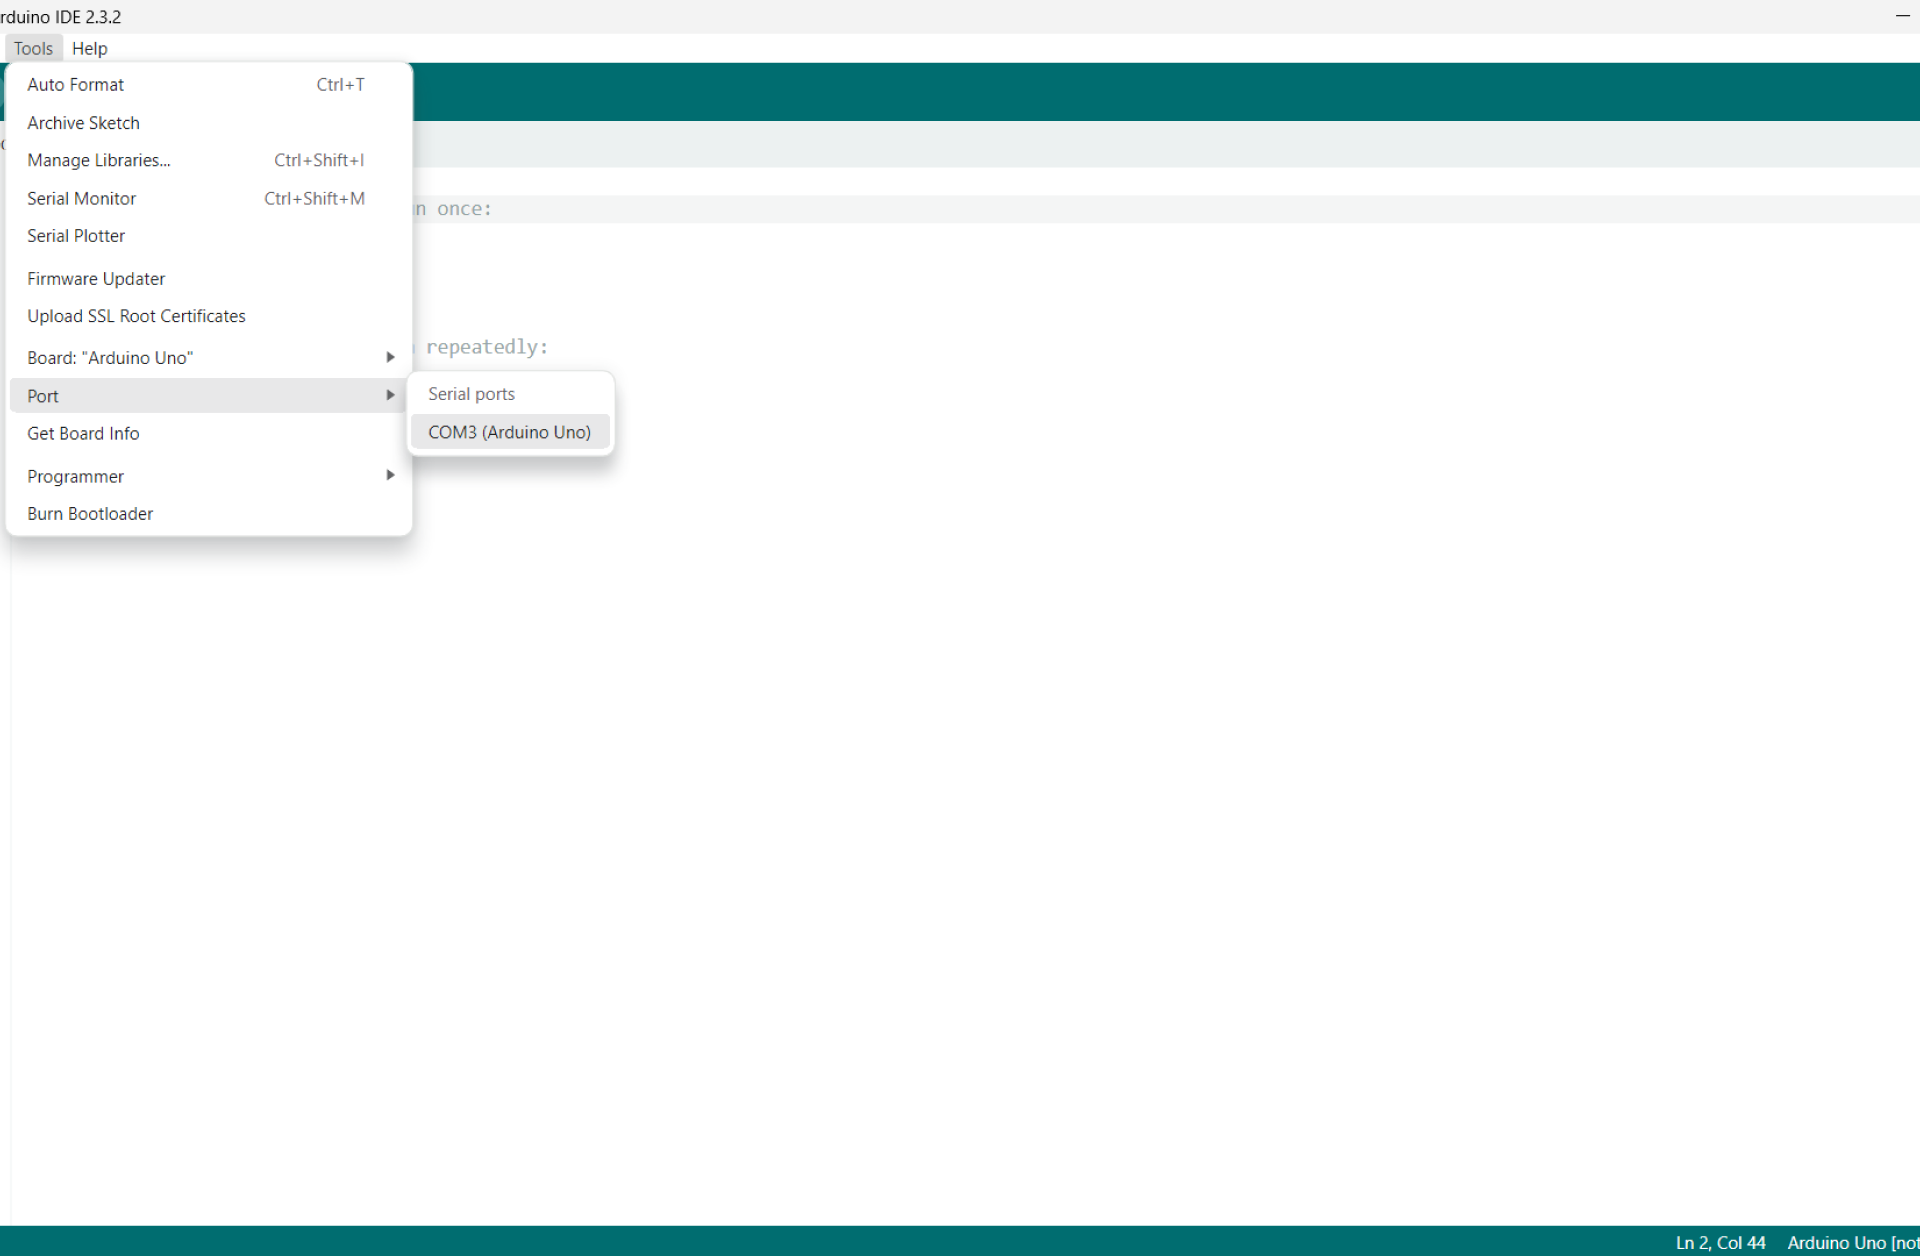
\includegraphics[width=0.8\linewidth]{P3/img/step 4.png}
			\caption{Step 4}
			\label{fig:Step 4}
		\end{figure}

		\begin{figure}[H]
			\centering
			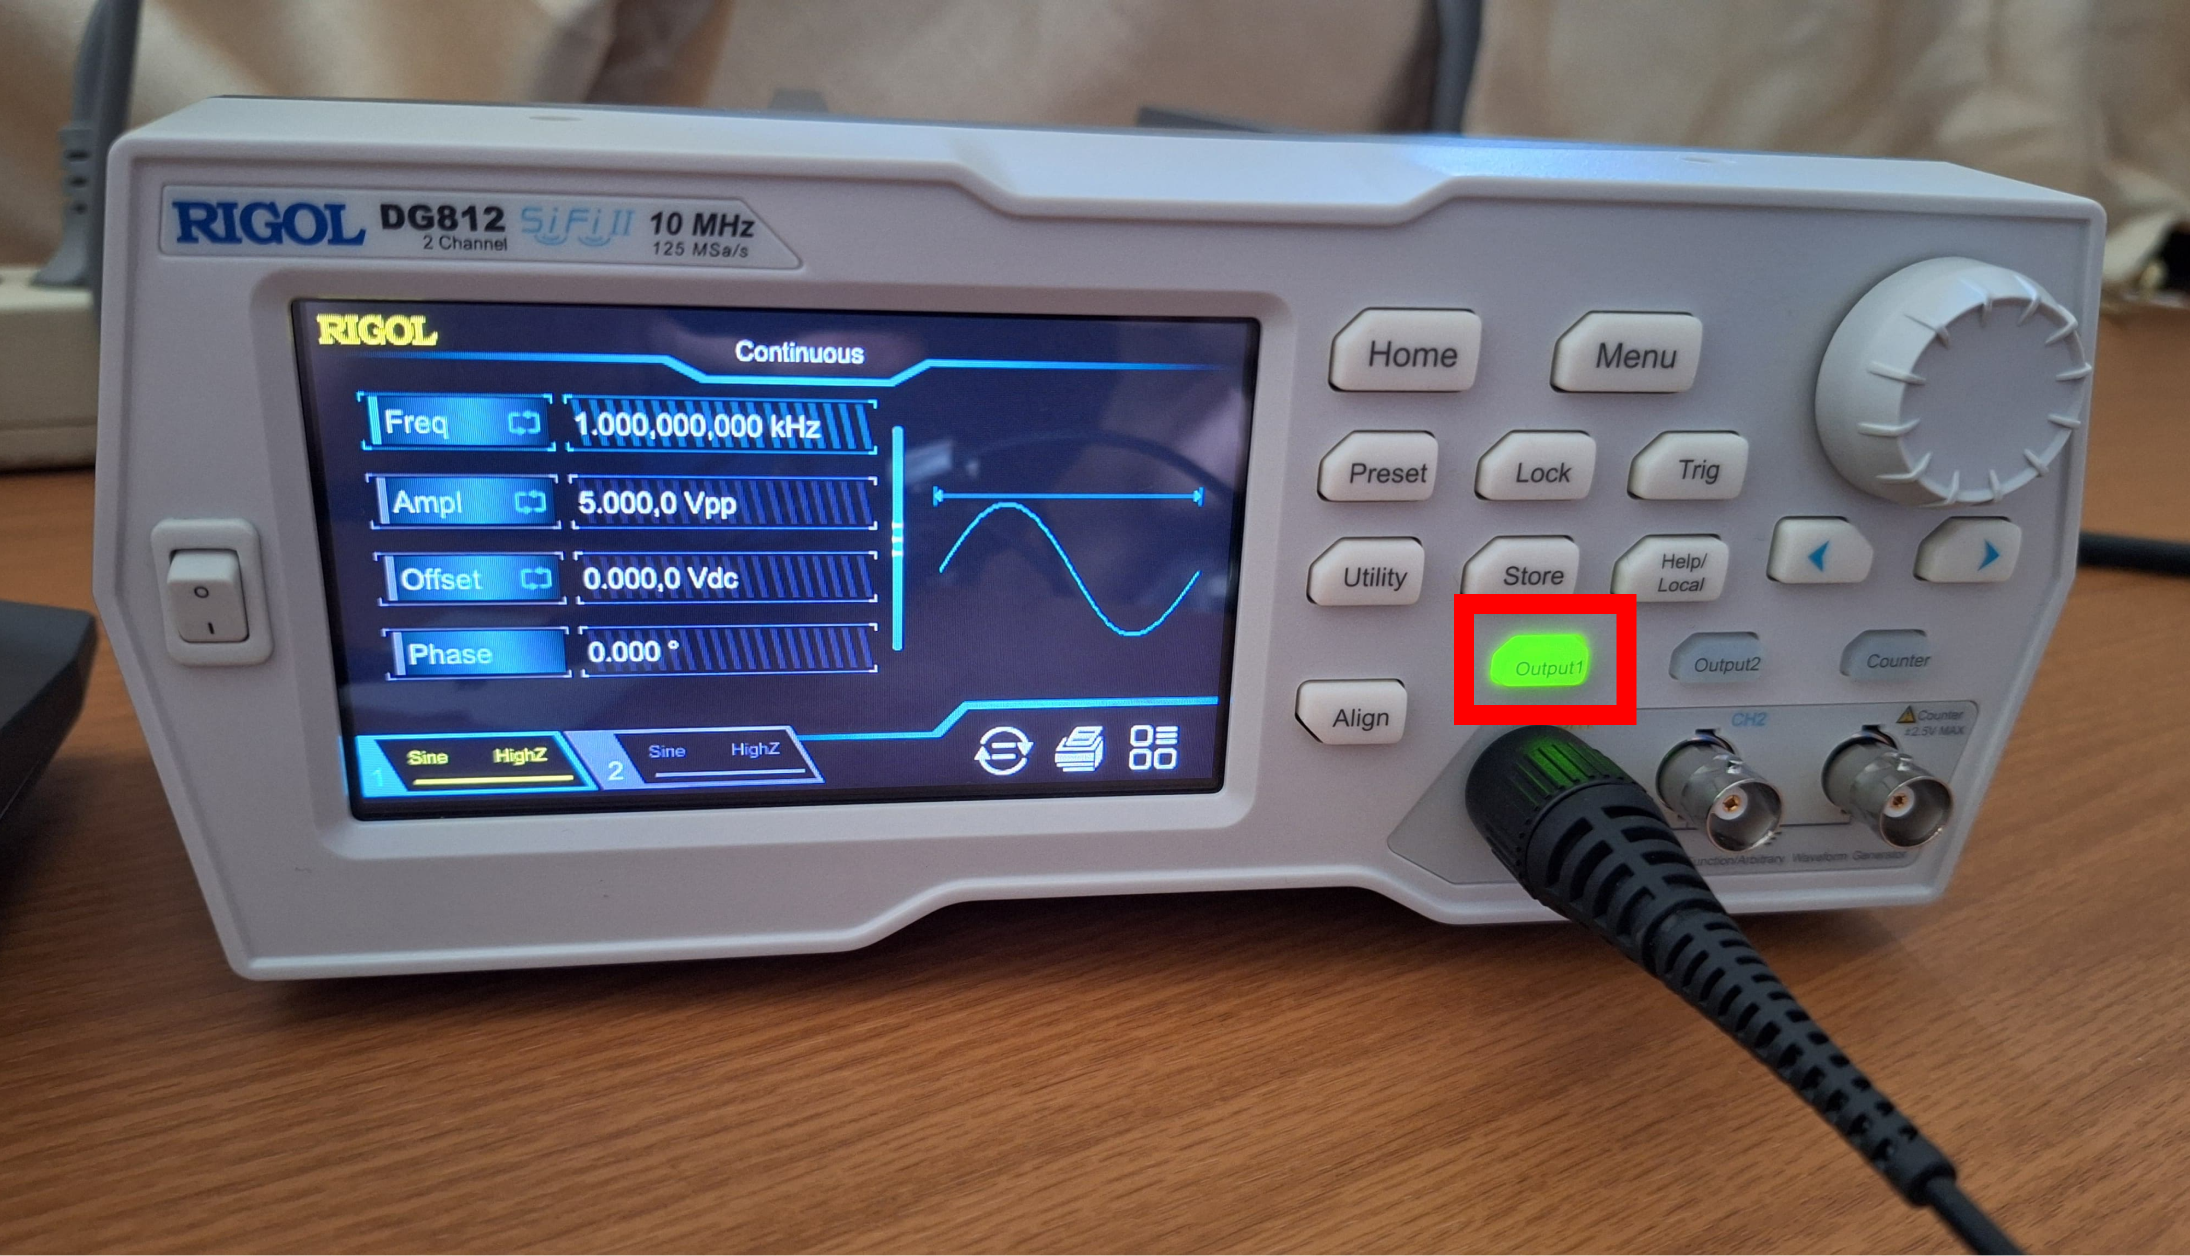
\includegraphics[width=0.8\linewidth]{P3/img/step 5.png}
			\caption{Step 5}
			\label{fig:Step 5}
		\end{figure}

		\begin{figure}[H]
			\centering
			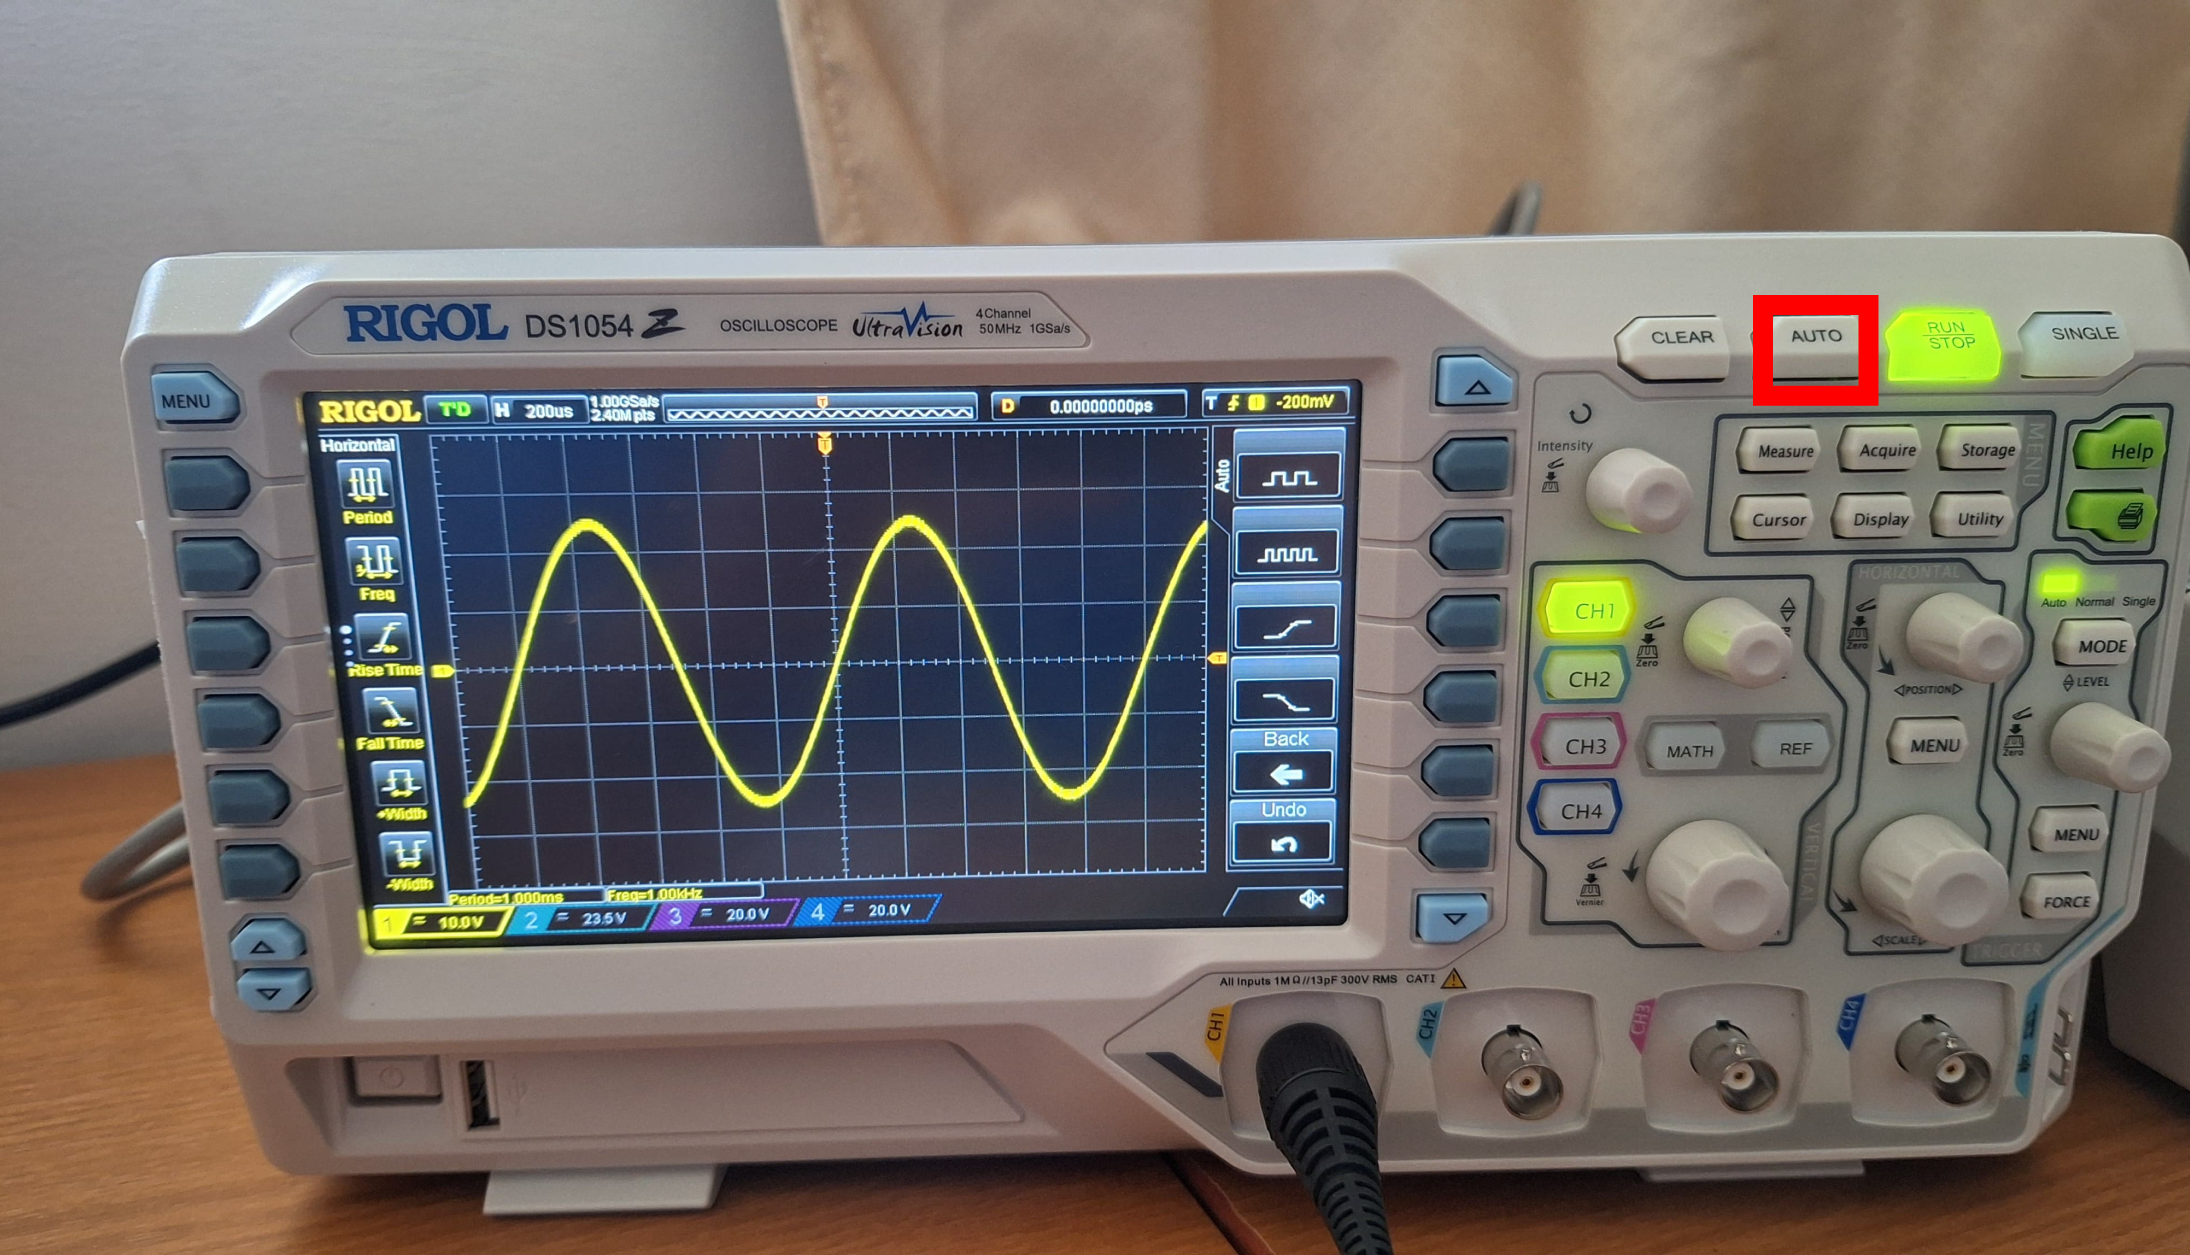
\includegraphics[width=0.8\linewidth]{P3/img/step 6.png}
			\caption{Step 6}
			\label{fig:Step 5}
		\end{figure}

        \item Buka Serial Plotter di pojok kanan atas pada Arduino IDE.
        \item Buka Serial Monitor di pojok kanan atas pada Arduino IDE.

    \end{enumerate}
\end{center}

\subsection{Percobaan 2}
\begin{center}
	\textbf{Konfigurasi Osiloskop}
	\begin{enumerate}
		\item Hubungkan kabel power ke osiloskop, lalu tekan tombol power untuk menyalakan Osiloskop. 
		\begin{figure}[H]
			\centering
			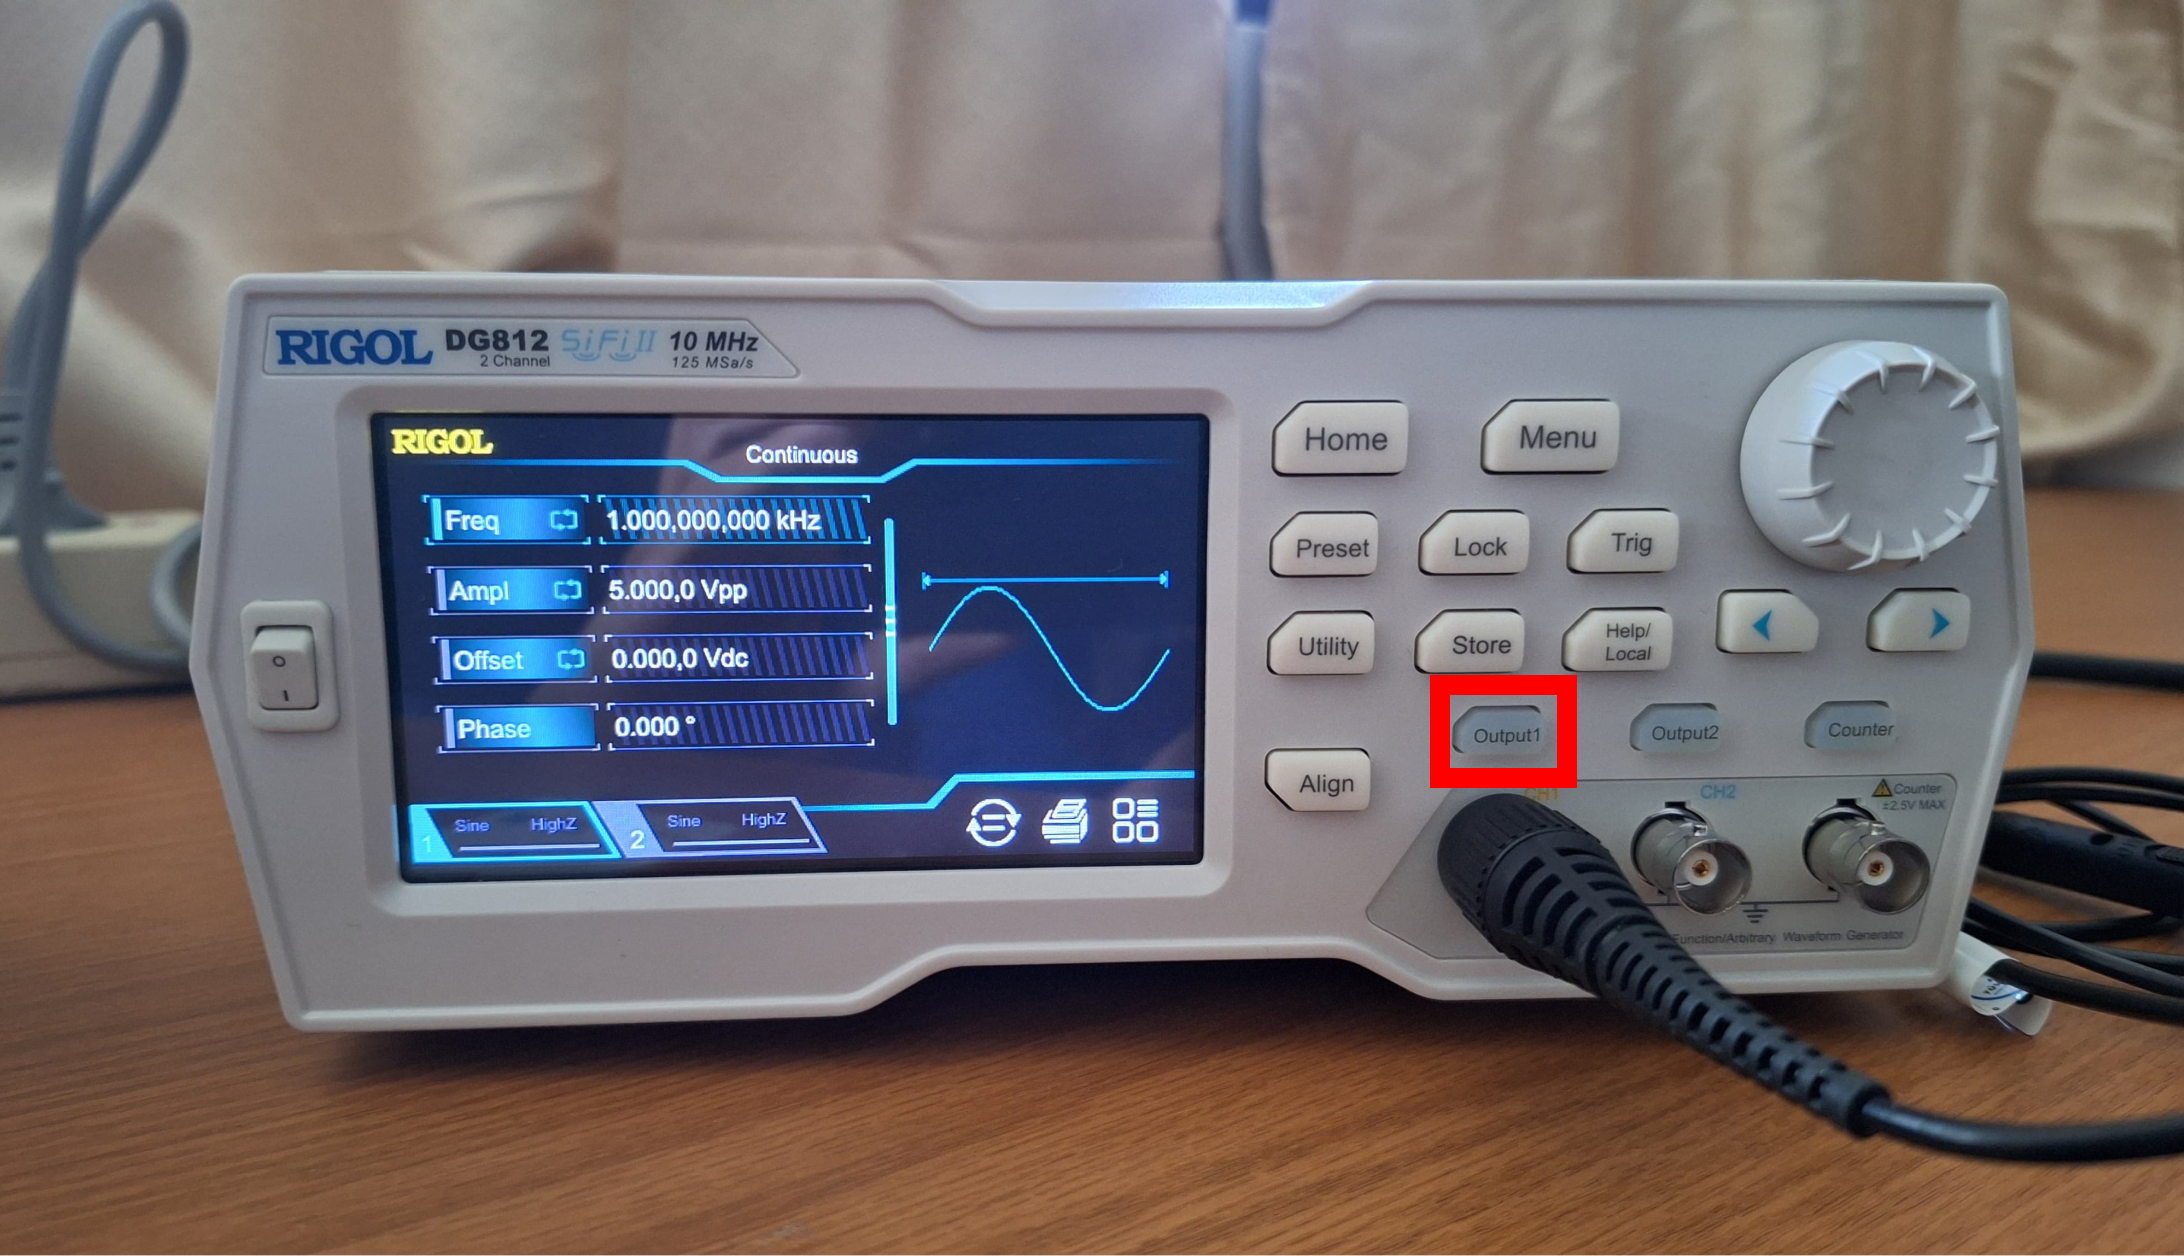
\includegraphics[width=0.8\linewidth]{P3/img/step 7.png}
			\caption{Step 1}
			\label{fig:Step 1(Step 1)}
		\end{figure}
		\item Hubungkan kabel probe pada channel 1. 
		\begin{figure}[H]
			\centering
			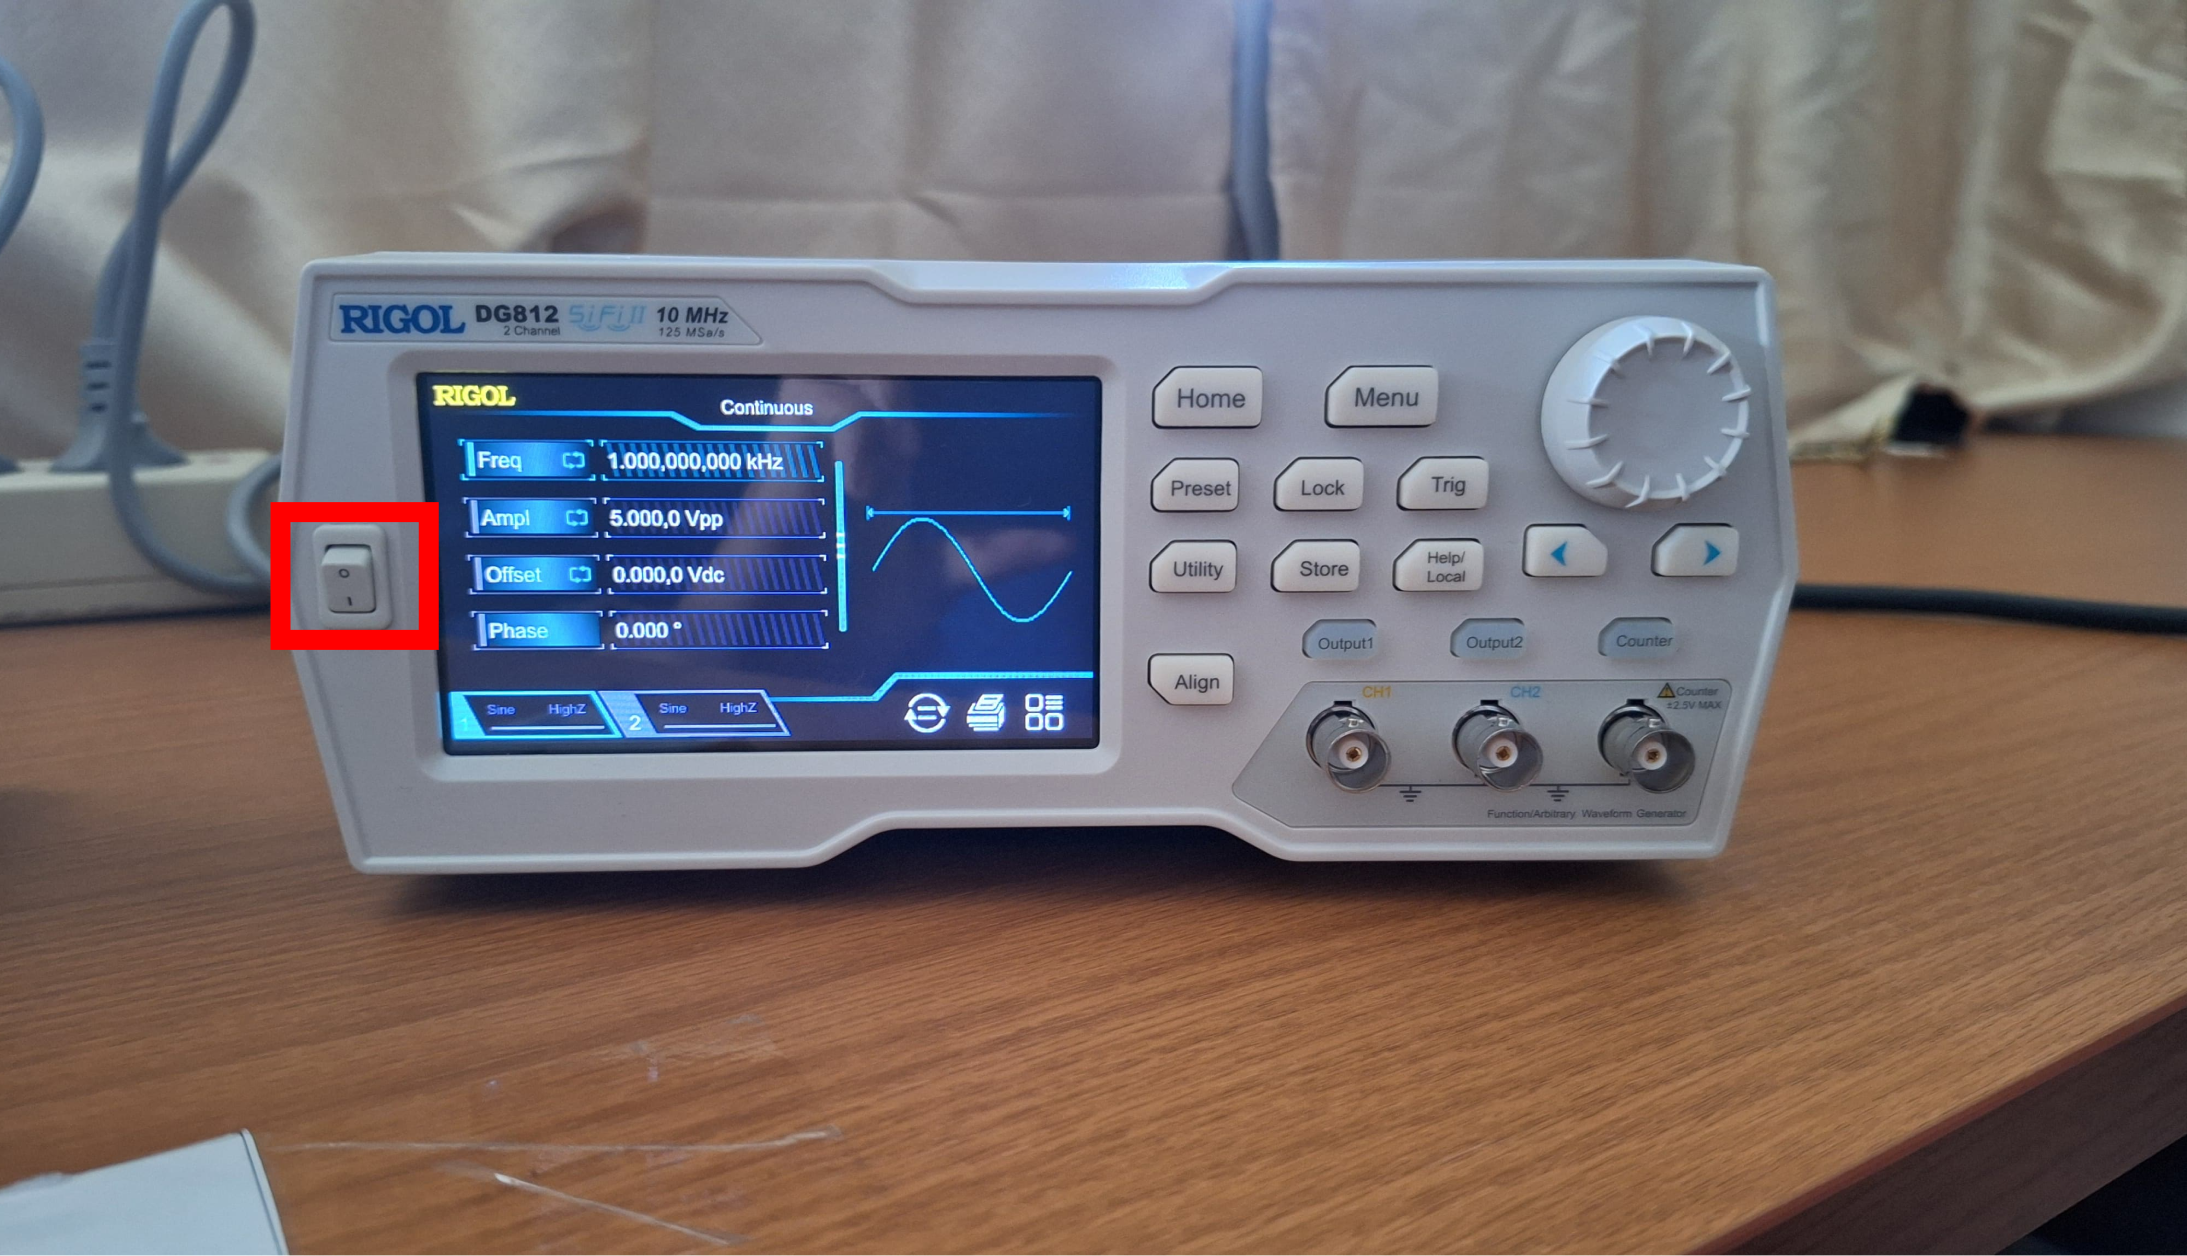
\includegraphics[width=0.8\linewidth]{P3/img/step 8.png}
			\caption{Step 2}
			\label{fig:Step 2(Step 2)}
		\end{figure}
		\item Hubungkan kabel output R2R Ladder dengan probe pengait osiloskop.
		\item Hubungkan kabel probe penjepit buaya osiloskop pada GND R2R Ladder.
		\item Klik AUTO pada Osiloskop.
		\item Bandingkan hasil sinyal yang ditampilkan oleh Serial plotter Arduino dengan Osiloskop.
	\end{enumerate}	
\end{center}

%===========================================================%
\section{Hasil yang didapat}
Memahami perbedaan hasil sinyal anlog yang diperoleh oleh Arduino dan Osiloskop.

%===========================================================%
\section{Kesimpulan}
Mengetahui hasil sinyal manakah yang lebih baik dihasilkan dari kedua perangkat \\Arduino dan Osiloskop.
